\documentclass{scrreprt} % <= Druckversion: "scrbook", Bildschirmversion: "scrreprt"
\newcommand\bcor{12mm} % <= Bindungskorrektur für Druckversion
\usepackage{osm-thesis}


\usepackage{ellipsis} % Leerraumoptimierung
\usepackage{booktabs} % Tabellenstriche unterschiedlicher Stärke
\usepackage{tabularx} % Automatische Zeilenumbrüche
\usepackage{tablefootnote}
\newcommand{\ra}[1]{\renewcommand{\arraystretch}{#1}}
\usepackage{minted} % Farbige Hervorhebung von Quellcode
\RequirePackage{csquotes} % Loaded later because of minted

\usepackage[multiple]{footmisc} % Trennung mehrerer Fußnoten durch Kommata
% Requires \usepackage[hyperfootnotes=false,...]{hyperref}, see https://tex.stackexchange.com/a/35060

\usepackage{wrapfig}
\usepackage{subcaption}

% Import SVG directly via Inkscape-pdf_tex-Export
\usepackage{import}
\graphicspath{{images/}}
\newcommand{\executeiffilenewer}[3]{%
	\ifnum\pdfstrcmp{\pdffilemoddate{#1}}%
	{\pdffilemoddate{#2}}>0%
	{\immediate\write18{#3}}\fi%
} 
\newcommand{\includesvg}[1]{%
	\executeiffilenewer{#1.svg}{#1.pdf}%
	{inkscape -z -D --file=#1.svg %
		--export-pdf=#1.pdf --export-dpi=72 --export-latex}%
	\input{#1.pdf_tex}%
}

% ABOUT
\newcommand{\hpitype}{Masterarbeit}
\newcommand{\hpiauthor}{Jan-Henrich Mattfeld}

% und Implementierung	
\newcommand{\hpititle}{Entwurf einer einheitlichen Middleware zur Policy-Durchsetzung in Multi-Cloud-Infrastrukturen}
\newcommand{\hpititleother}{Design and Implementation of a Unified Middleware for Policy Enforcement in Multi-Cloud Infrastructures} % <= das Studienreferat verlangt einen deutschen UND englischen Titel

\newcommand{\hpisupervisor}{Max Plauth, Prof.\,Dr.\,Andreas Polze}
\newcommand{\hpichair}{Fachgebiet für Betriebssysteme und Middleware}
\newcommand{\hpiexternalsupervisor}{}
\newcommand{\hpiexternal}{}
\newcommand{\hpidate}{\today}

% DOCUMENT
%\KOMAoption{draft}{true} % <= z.B. zum "Debuggen" der Overfull-Boxes und schnellerem Kompilieren https://tex.stackexchange.com/a/49369
\bibliography{literature/bibliography}

\begin{document}
	\selectlanguage{ngerman}

	% Einband
	\pagenumbering{alph}
	\ifisbook\include{content/coverpage}\fi
	\ifisbook\cleardoubleemptypage\fi

	% (Haupt-)Titelseite, Abstract, ggf. Danksagung & Inhaltsverzeichnis
	\pagenumbering{roman}
	\include{content/titlepage}
	\ifisbook\cleardoubleemptypage\fi
	% \null\vfil
\begin{otherlanguage}{ngerman}
\begin{center}\textsf{\textbf{\abstractname}}\end{center}

Cloud-Ressourcen spielen eine entscheidende Rolle in den aktuellen und zukünftigen IT-Strategien von Unternehmen aller Größen. Gleichzeitig entstehen zentrale Herausforderungen in Hinblick auf Vertraulichkeit und Zuverlässigkeit, sowie Portabilität der eigenen Daten und Anwendungen. Mit dem Inkrafttreten der Datenschutz-Grundverordnung und immer neuen Datenlecks ist das Thema hochaktuell.

Durch die intelligente Kombination von Private- und Public-Cloud-Infrastruktur treten wir diesen Herausforderungen entgegen. Wir geben einen Überblick über aktuelle kommerzielle und akademische Multi-Cloud-Projekte. Dabei identifizieren wir fehlende SLA- und Cloud-Schnittstellen-Standards als größte Risiken.

Als Lösungsvorschlag entwickeln wir einen Multi-Cloud-Anwendungs-Broker auf den Ebenen IaaS und CaaS. Dabei dient das TOSCA-Simple-Schema zur Anwendungs- und SLA-Spezi\-fi\-ka\-tion. Wir diskutieren den Aufwand der Cloud-Teststellungen und den Einsatz der Multi-Cloud-Bibliothek Apache Libcloud. Die Leistungsfähigkeit der Lösung demonstrieren wir anschließend in einem Testaufbau mit OpenStack, AWS, Docker und Hyrise-R.

Wir versetzen Cloud-Kunden in die Lage, ihre Anforderungen anbieter- und technikunabhängig zu formulieren und durchzusetzen. Unsere Lösung automatisiert die Einhaltung von Datenschutz-, Qualitäts- und Kostenzielen. Damit ist das Projekt einzigartig und ergänzt die bisherigen Beiträge im SSICLOPS-Kontext.

\end{otherlanguage}
\vfil\null




	\tableofcontents
	\cleardoublepage

	% Textteil
	\pagenumbering{arabic}
	\chapter{Einleitung}

Cloud-Angebote sind allgegenwärtig und werden mittlerweile von einer Mehrzahl deutscher Unternehmen genutzt. Laut \emph{Statista} setzten bis 2016 mindestens fünfundsechzig Prozent aller Betriebe entsprechende Lösungen ein \cite{bitkom:2017:cloud-nutzung-unternehmen}. Besonders gefragt sind Infrastrukturdienste, wie Rechenleistung und Speicher. Gleich darauf folgen Softwareangebote und E-Mail-Hosting. Etwas abgeschlagen bleiben Plattformdienste wie Datenbanken und Ausführungsumgebungen \cite{destatis:2016:cloud-nutzung-unternehmen-einsatzzweck}. Der Trend zur Cloud wird sich vermutlich fortsetzen: So vervierfacht sich das prognostizierte Marktvolumen mit Cloud-Services bis 2020 auf über sechzehn Milliarden Euro allein im deutschen B2B-Markt \cite{isg:2017:cloud-ausgaben-2020}.

Cloud-Angebote sind für Unternehmen aller Größen attraktiv: Die Anschaffung eigener Infrastruktur entfällt, genauso wie deren Wartung durch eigenes Personal. Stattdessen lassen sich Ressourcen und Anwendungen einfach per Self-Service buchen und sind anschließend über das Internet von überall erreichbar. Der Umfang gebuchter Leistungen lässt sich meist frei skalieren. Da die Angebote oft in kleinem Takt und verbrauchsgenau abgerechnet werden, ergeben sich so theoretisch Vorteile bei Flexibilität und Kosteneffizienz.

Demgegenüber stehen Vorbehalte bezüglich Datenschutz, denn die gemietete Infrastruktur teilen sich mehrere Kunden. Durch Sicherheitslücken wie \emph{Spectre} und \emph{Meltdown} werden eigentlich geschützte Speicherbereiche angreifbar \cite{Kocher2018spectre, Lipp2018meltdown}. Nach aktuellem Stand existierten diese Lücken mehr als ein halbes Jahr in fast jedem x86-System, und damit in fast jeder Cloud \cite{techcrunch:2018:spectre-meltdown-tier-2-cloud-vendors}. Eine sichere Mandantentrennung war also nicht mehr gewährleistet \cite{aws:2018:security-bulletin}. Aber auch durch Unachtsamkeit werden Cloud-Datenspeicher immer wieder der Öffentlichkeit zugänglich \cite{upguard:2017:breach-alteryx, upguard:2017:breach-centcom, kromtech:2018:breach-fedex}.

Zugleich fordert aktuelle Gesetzgebung wie die Datenschutz-Grundverordnung unter anderem die Verarbeitung von personenbezogenen Daten europäischer Kunden ausschließlich innerhalb der EU \cite{eu:2016:bdsvg}. Gut neunzig Prozent aller Unternehmen achteten folglich bei der Auswahl eines Cloud-Providers auf Rechts- und Server-Standorte in Deutschland \cite{gartner:2017:cloud-market}. Auch vorhandene Softwarelizenzen können den Umzug verhindern. Zum Beispiel Oracle- und Microsoft-OEM-Lizenzen verbieten die Übertragung in eine Cloud-Umgebung \cite{microsoft:2017:licensing, oracle:2018:licensing}. So müssen möglicherweise Teile der Infrastruktur lokal vorgehalten werden.

Für gut fünfzig Prozent der interessierten Unternehmen außerdem unabdingbar: individuelle Dienstgütevereinbarungen, sogenannte \emph{Service Level Agreements (SLAs)} \cite{bitkom:2017:cloud-nutzung-unternehmen-auswahlkriterien}. Dies lässt jedoch einige der weltweit größten Cloud-Anbieter außen vor -- Amazon und Microsoft teilen sich seit 2016 über fünfzig Prozent des weltweiten Umsatzes mit Infrastrukturdiensten \cite{gartner:2017:cloud-market}. Die Vertragsbedingungen beider Anbieter sind jedoch nicht verhandelbar.

Laut Gartner wollen daher 70 Prozent aller Unternehmen bis 2019 eine Multi-Cloud-Strategie umsetzen \cite{gartner:2017:cloud-market-multicloud-trend}. Auch das EU-geförderte Forschungsprojekt \emph{Scalable and Secure Infrastructures for Cloud Operations (SSICLOPS)} identifiziert Multi-Cloud-Umgebungen als zukünftigen Treiber des ITK-Markts \cite{ssiclops:2015:d6.1-project-presentation}. Zusätzlich zu einer privaten Cloud werden hierbei auch Dienste aus weiteren öffentlichen Angeboten genutzt. Vorteil ist eine höhere Flexibilität, um für jede Anforderung die ideale Cloud wählen zu können. Kriterien sind zum Beispiel die Einhaltung gesetzlicher Anforderungen, spezielle SLAs, höhere Ausfallsicherheit und die Preisgestaltung der Anbieter. Multi-Cloud birgt aber auch einige Herausforderungen:

\begin{itemize}
	\item Portabilität eigener Anwendungen
	\item Cloud-Provider-spezifisches Know-how
	\item Höherer IT-Verwaltungsaufwand der Ressourcen
	\item Managementaufwand, wie der Vergleich von Compliance-Richtlinien
	\item Keine oder geringere preisliche Skaleneffekte
	\item Überwachung der heterogenen Cloud-Landschaft
	\item Durchsetzung der eigenen Sicherheits- und Datenschutzrichtlinien
\end{itemize}

Um diese Herausforderungen automatisiert abzumildern, eignet sich eine \emph{Cloud-Management-Plattform (CMP)} mit integriertem Anwendungs-Broker. Deren Marktsituation ist allerdings unübersichtlich und in großer Bewegung. Bereits im letzten Jahr wurden einige vielversprechende Lösungen von Cloud-Infrastruktur-Providern aufgekauft \cite{gartner:2017:cloud-market-multicloud-trend}. Die CMPs sind nun selbst Software-as-a-Service-Angebote und proprietär. Die eigentlichen Vorteile Flexibilität und Unabhängigkeit werden so ad absurdum geführt.

Unabhängige Lösungen sind mehrheitlich ausgelaufene akademische Forschungsprojekte. Auf den aktuellen Cloud-Markt und technische Neuerungen wie Container sind diese nicht mehr anwendbar. Aufgrund der vorherigen Forschungsergebnisse ergibt sich jedoch folgende Hypothese:

\begin{verse}
	{\emph{Eine unabhängige, auf offenen Standards basierende CMP kann die \newline Vorteile der Cloud mit aktuellem Datenschutz vereinen.}}
\end{verse}

Im Rahmen dieses Projektes entwickeln wir einen Multi-Cloud-Broker. Alle Ergebnisse basieren auf Open-Source-Technologien und sollen, wenn möglich, an die Ursprungsprojekte zurückfließen. Der Broker soll Organisationen und Unternehmen als Cloud-Nutzer emanzipieren und besonders den kommerziellen Wert der Lösung herausstellen.

Da SLAs und weitere Rahmenbedingungen oft nicht verhandelbar sind, muss die Optimierung der Cloud-Nutzung in Eigenregie erfolgen.  Die vorgestellte CMP erlaubt die Nutzung bestimmter Anbieter, obwohl SLAs  nicht eingehalten werden: Zum Beispiel lässt sich eine höhere Ausfallsicherheit durch Kombination mehrerer Anbieter erreichen. Nebenbei entsteht so ein Notfallplan zum Weiterbetrieb bei Ausfall oder Kündigung eines Cloud-Providers.

Das folgende Kapitel klassifiziert Cloud-Angebote anhand bestimmter Eigenschaften und Service-Ebenen. Außerdem geben wir eine Einführung in datenschutzrechtliche Fragen und Risiken in Zusammenhang mit Cloud-Bereit\-stel\-lungs\-model\-len.

Anschließend entwickeln wir passende Policys und entsprechende Schemata. Diese sollen von dem eigens entwickelten Multi-Cloud-Broker verwendet werden. Er verteilt auch bestehende, nicht Cloud-native, Anwendungen über verschiedene Cloud-Provider auf IaaS- und CaaS-Ebenen und optimiert die Cloud-Landschaft anschließend fortlaufend. Dabei beachtet er SLAs und Datenschutzanforderungen. Für diesen Vorschlag bewerten wir akademische und kommerzielle Projekte mit ähnlicher Zielsetzung.

Der Implementierungsteil vergleicht verschiedene Multi-Cloud-Bibliotheken. Auf Basis von Apache \emph{Libcloud} entwickeln wir eine CMP, die das Multi-Cloud-Brokering übernimmt. Auch Implementierungshürden und Besonderheiten der verschiedenen Clouds werden beschrieben. Als Beispielanwendung dient dabei die verteilte Forschungsdatenbank \emph{Hyrise-R}. Auch die Entstehung eines \emph{OpenStack}-Testbeds als Beispiel einer Private-Cloud wird besprochen. Es folgt eine abschließende Bewertung des Konzepts.

	\chapter{Hintergrund -- Chancen und Herausforderungen in der Cloud}

Dieses Kapitel definiert die grundlegenden Charakteristika eines Cloud-Dienstes, die verschiedenen Service-Ebenen, Liefermodelle, Akteure und ihre Verantwortlichkeiten. Aus diesen Definitionen entwickeln sich zwei grundlegende Herausforderungen der Cloud-Nutzung:

\begin{enumerate}
	\item Datenschutz/Vertraulichkeit
	\item Portabilität von Daten und Anwendungen
\end{enumerate}

Je nach Cloud-Nutzung ergeben sich hierfür verschiedene Lösungsansätze, die im weiteren Verlauf gegeneinander abgegrenzt werden.


\section{Eigenschaften eines Cloud-Dienstes}

Unabhängig von Liefer- und Servicemodell zeichnet sich ein Cloud-Dienst durch bestimmte Merkmale aus. Konkret definieren übereinstimmend \emph{NIST Cloud Computing Reference Architecture}, \emph{IETF} und \emph{BSI-Grundschutzkatalog} \cite{nist:2011:reference-architecture, ietf:2015:reference-framework, bsi:2014:grundschutz} folgende Eigenschaften:

\begin{description}
	
	\item[On-demand Self-Service] Ressourcen werden vom Cloud-Kunden selbstständig über ein Portal oder eine Webschnittstelle angefordert und anschließend automatisch provisioniert.
	
	\item[Breitbandzugriff] Die gemieteten Ressourcen werden über ein Netzwerk, typischerweise das Internet, bereitgestellt. Der Zugriff erfolgt über Standardschnittstellen wie HTTP; kann also von überall erfolgen und ist im Regelfall nicht auf bestimmte Geräte oder Software beschränkt.
	
	\item[Geteilte Infrastruktur] Die zugrunde liegenden physischen Ressourcen werden virtualisiert und flexibel unter mehreren Kunden aufgeteilt. Die vorhandene Hardware wird so möglichst optimal ausgelastet. Gleichzeitig ergeben sich hierdurch Datenschutzbedenken; die Daten einzelner Mandaten müssen streng getrennt sein.
	
	\item[Elastizität] Durch einen hohen Grad an Automatisierung werden Ressourcen zeitnah zur Verfügung gestellt. Lastspitzen können ohne manuelle Eingriffe abgefangen werden.
	
	\item[Messbarkeit] Die Ressourcennutzung ist messbar und wird kontinuierlich überwacht. Abgerechnet wird zum Beispiel nach CPU-Zeit, Speicherkapazität oder Anzahl genutzter IP-Adressen.
	
\end{description}

Von klassischem IT-Outsourcing grenzt es sich durch Self-Service, Skalierbarkeit und geteilte Infrastruktur ab. Diese Eigenschaften bieten Kunden theoretisch Flexibilität und Kostenvorteile. In der Lösungssuche sollen diese positiven Aspekte möglichst erhalten bleiben.


\section{Service-Ebenen}

Je nach Auswahl des Cloud-Angebots lassen sich verschiedene Kernebenen unterscheiden. Diese bauen jeweils aufeinander auf und verbergen die Komplexität der darunterliegenden Ebenen. Je weiter sich die Abstraktion von der physischen Ebene entfernt, desto weniger lässt sich das Angebot durch den Kunden anpassen:

\begin{description}
	
	\item[Infrastructure as a Service (IaaS)] Die klassische Bereitstellung von Infrastruktur wie virtuellen Maschinen, Speicherplatz und Netzwerkdienstleistungen. Der Kunde ist hier selbst für die Administration zuständig, muss also Einrichtung und Wartung von Betriebssystemen, Treibern und Middleware selbst verantworten.
	
	\item[Container as a Service (CaaS)] Variante von IaaS, bei dem eine Laufzeitumgebung für Container bereitgestellt wird. In diesen sind alle Abhängigkeiten der Gastanwendung vorinstalliert und laufen auf dem bereits initialisierten Kernel des Hosts. Vorteil ist eine höhere Elastizität durch geringeren Overhead. Im Folgenden ist bei der Erwähnung von IaaS immer auch CaaS inkludiert.
	
	\item[Platform as a Service (PaaS)] Hier übernimmt der Cloud-Provider die Bereitstellung der zuvor genannten Bestandteile. Der Kunde betreibt auf dieser Ebene eine selbst erstellte Anwendungssoftware. Über Bibliotheken und Schnittstellen des Cloud-Providers greift er auf Laufzeitumgebungen, Datenbanken und Entwicklungswerkzeuge zu.
	
	\item[Function as a Service (FaaS)] Auch als \emph{Serverless-Computing} populär: Entgegen dem Namen arbeiten auch hier noch Server, diese sind für den Kunden jedoch weitestgehend unsichtbar. Es stellt eine Evolution des PaaS-Modells dar und ist besser als FaaS beschrieben -- der Kunde lädt nur noch Quellcode in die Cloud. Dieser wird nun Ereignis-getrieben ausgeführt, skaliert und abgerechnet. Im Gegensatz zu vielen PaaS-Angeboten fallen im Ruhebetrieb keine weiteren Kosten an \cite{crisp:2016:serverless-infrastructure}.
	
	\item[Software as a Service (SaaS)] Eine bestehende Anwendungssoftware wird komplett vom Cloud Provider bezogen. Die Verantwortlichkeit des Kunden beschränkt sich meist auf kleinere Anpassungen, Nutzerverwaltung und das Einspielen eigener Daten.
	
\end{description}

Besonders interessant für eigene Entwicklungen im Rahmen des \emph{SSICLOPS}-For\-sch\-ungs\-kon\-tex\-tes sind dabei die Ebenen IaaS und CaaS \cite{ssiclops:2015:d6.1-project-presentation}. Sie bieten genug Flexibilität, um die Fragestellung mit folgenden Produkten zu erproben:

\begin{enumerate}
	\item \emph{OpenStack} als zentraler Infrastrukturprovider
	\item Die verteilte Forschungsdatenbank \emph{Hyrise-R} als Beispielanwendung
\end{enumerate}

Cloud-Provider bieten darüber hinaus weitere Hilfs- und Verwaltungsdienste. Diese betreffen vor allem Konfiguration, Provisionierung, Monitoring und Abrechnung. Hierzu zählen aber auch Sicherheit, Vertraulichkeit und Portabilität. Diese drei Querschnittsthemen sollen im Zusammenhang mit den Dienstebenen weiter untersucht werden.

Die \emph{NIST}-Klassifizierung unterscheidet hier speziell weitere, teils externe, Akteure wie Cloud-Auditoren und -Carrier \cite{nist:2011:reference-architecture}. Dieser Einteilung folgt die Arbeit nicht. Stattdessen konzentriert sie sich auf die direkte Beziehung zwischen Cloud-Kunden und -Provider. Beide haben Risiken und Verantwortlichkeiten, die im nächsten Abschnitt besprochen werden.


\section{Risiken}

Moderne IT-Infrastruktur ist hochkomplex. Allein hierdurch ergibt sich ein großes Potenzial für Bedrohungen. Im Cloud-Computing steigt das Risiko durch gemietete und geteilte Infrastruktur weiter \cite{csa:2016:cloud-top-threats, Pearson:2010:issues-arising-cloud, 2011:takabi:security-challenges}. Zusätzlich zu allgemeinen Risiken sollen mögliche Auswirkungen auf folgende Eigenschaften beschrieben werden:

\begin{enumerate}
	\item Verfügbarkeit
	\item Vertraulichkeit
	\item Integrität
	\item Portabilität
\end{enumerate}

Abhängig vom Einsatzzweck des geplanten Cloud-Services resultieren die Fragen: Welche Informationen und Prozesse müssen geschützt werden, welche Bedrohungen sind zu erwarten? Damit ist nicht nur Sicherheit gemeint, sondern alle Risiken, die den Erfolg eines Cloud-Projektes oder einer Organisation darüber hinaus bedrohen. Möglicher Schaden muss im Voraus berechnet werden. Zu verarbeitende Daten sollten kategorisiert werden; dem \emph{BSI} folgend sind diese vier Abstufungen denkbar \cite{bsi:2014:Anforderungskatalog}:

\begin{enumerate}
	\item Privat- , Geschäfts- und Dienstgeheimnisse gemäß \emph{§§\,203} und \emph{353\,b StGB}
	\item Personenbezogene Daten gemäß \emph{§\,3 Absatz\,1 BDSG}
	\item Verschlusssachen
	\item Sonstige Daten (weder Kategorie 1, noch 2, noch 3)	
\end{enumerate}

Verschlusssachen der Kategorie drei meint hier alle Daten, deren Verlust, Veränderung oder unrechtmäßige Herausgabe sich nachteilig auswirken könnte. Die Abgrenzung der letzten beiden Kategorien erscheint oft schwierig, muss jedoch für jeden betriebenen Cloud-Service abgewogen werden.

Diese Arbeit konzentriert sich auf die Risiken, die direkt von Cloud-Kunden und \mbox{-Providern} auf den Ebenen IaaS und PaaS beeinflusst werden können. So ist zum Beispiel die Sicherheit der Client-Geräte, von denen auf die Cloud-Dienste zugegriffen wird entscheidend, aber nicht Teil dieser Betrachtung.

Aus der Datenkategorie ergeben sich Anforderungen an die Risikoanalyse. Je höher und je wahrscheinlicher ein potenzieller Schaden, desto aufwendiger und teurer sollte die Absicherung ausfallen. Grundsätzlich lassen sich zwei Kategorien von Risikofaktoren unterscheiden \cite{monjur:2017:security-taxonomy}:

\begin{itemize}
	\item Menschlich
	\item Technisch
\end{itemize}

Menschliche Fehlhandlungen sind entweder absichtlich oder unabsichtlich. Dies können Fehlinterpretation von SLAs, Manipulationen, Angriffe durch \emph{Social-Engineering} oder schlicht Inkompetenz sein. Im Cloud-Computing treten diese Risiken verstärkt auf, da die Infrastruktur von Dritten betreut wird. Auch Gesetzesänderungen zählen zu diesen Risiken. Viele lassen sich durch passende Standardprozesse, Notfallpläne, Rechtemanagement und Audits vermindern.

Technisch gilt Ähnliches: Klassische Risiken, wie der Ausfall von Hardware, wird vom Cloud-Provider vor dem Kunden verborgen. Speziell auf Cloud-Projekte bezogen eröffnen sich aber auch neue Angriffsflächen wie die Cloud-Plattform selbst. Die Virtualisierungsebene kann durch mangelhafte Mandantentrennung Datenlecks öffnen. Viele Cloud-Provider arbeiten mit proprietären Protokollen, die Portabilität ist also eingeschränkt. Umso herausfordernder wird ein Notfallplan, der den Ausfall des Anbieters abfangen soll.

All diese Risiken müssen durch SLAs und Policys abgebildet werden. Diese sollten maschinenlesbar sein, um automatisiert angewandt und überprüft zu werden. Detaillierte Leitfäden hierzu bieten BSI und CSA \cite{bsi:2014:Sicherheitsrichtlinie, csa:2015:star}. Insgesamt hängt das Risiko stark vom Bereitstellungsmodell ab, also von Standort und Nutzerkreis der Infrastruktur.


\section{Bereitstellungsmodelle und Multi-Cloud-Architekturen}

Cloud-Angebote können von öffentlichen Anbietern oder intern bereitgestellt werden. Weiter differenzieren lassen sich die Angebote nach Nutzerkreis, mit dem die Infrastruktur geteilt wird und Anzahl der genutzten Clouds \cite{petcu:2014:cloud-taxonomy, grozev:2014:cloud-taxonomy}:

\begin{description}
	
	\item[Public Cloud] Alle Leistungen werden von einem öffentlichen Anbieter bezogen. Dies sind zum Beispiel Amazon, Microsoft und Google. Die Infrastruktur wird unter mehreren Kunden flexibel aufgeteilt.
	
	\item[Private Cloud] Eine eigen- oder fremd-betriebene Infrastruktur mit exklusivem Zugriff für einen Kunden. Wird die Private Cloud im eigenen Datencenter betrieben, erhalten Kunden größtmögliche Vertraulichkeit. Gleichzeitig müssen aber Überkapazitäten vorgehalten werden, wodurch der Kostenvorteil kleiner als bei Nutzung öffentlicher Angebote ausfallen kann.
	
	\item[Hybrid Cloud] Heterogene Infrastruktur mit Bestandteilen in privaten und öffentlichen Cloud-Umgebungen. Die öffentliche Cloud übernimmt hier oft die Speicherung großer Datenmengen und das Abfangen von Lastspitzen.
	
	\item[Community-Cloud] Ein Zusammenschluss von Unternehmen, Behörden oder For\-sch\-ungs\-ein\-rich\-tun\-gen, die gemeinsam eine Cloud-Infrastruktur betreiben. Die beteiligten Cloud-Anbieter bilden eine freiwillige \emph{Föderation} der gemeinsamen Ressourcen.
	
	\item[Multi-Cloud] Eine Erweiterung der Hybrid Cloud: Die Leistungen werden nicht nur aus einer privaten und einer öffentlichen Cloud bezogen, sondern explizit aus mehreren. Wichtiger Unterschied zur Föderation: Die Multi-Cloud-Umgebung wird vom Cloud-Anwender initiiert und verwaltet. Beteiligte Cloud-Provider wirken nicht aktiv mit und sind sich ihrer Partizipation meist nicht einmal bewusst.
	
\end{description}

Von allen beschriebenen Bereitstellungsmodellen ist die Multi-Cloud am flexibelsten. Je nach technischen und nicht-funktionalen Anforderungen können Bestandteile der Cloud-Anwendungen in einer möglichst passenden Umgebung ausgeführt werden. Der Aufwand ist in diesem Modell allerdings auch am höchsten, denn der Auswahlprozess für einen Cloud-Provider muss für alle Anbieter einzeln durchlaufen werden.

Hierbei werden die Rahmenbedingungen geprüft; unter anderem Kosten, Standort der Rechenzentren und anwendbare Gesetzesgrundlage. Hinzu kommen technische Herausforderungen, da die Portabilität von Daten und Anwendungen zwischen verschiedenen Cloud-Providern oft eingeschränkt ist.

Um eine automatisierte Bewertung der Cloud-Angebote vorzunehmen, müssen die Anforderungen möglichst genau spezifiziert werden. Dazu dienen Policys und SLAs. Der folgende Abschnitt zeigt die wichtigsten Beispiele und erläutert ihre Bedeutung im Kontext der Arbeit.


\section{Policys, SLAs und Optimierungsgrößen}

Cloud-Nutzer und -Provider haben gegenseitige Erwartungen, die abgestimmt werden müssen. Innerhalb von Unternehmen gelten außerdem bestimmte Regeln zum Umgang mit Informationen (\emph{Compliance}), angelehnt an die Gesetzeslage und externe Zertifizierungen wie ISO 27001 \cite{iso:2013:27001}. Über die gesetzlichen Regelungen hinaus kann ein Unternehmen weitere Ziele setzen: Kosteneinsparungen oder der Einsatz klimafreundlicher Energie.

Dieser Abschnitt definiert die verschiedenen Formen für den späteren Einsatz im Multi-Cloud-Broker. Er liefert Verweise zu Standards und entwickelt Beispiele für den späteren Prototyp. Wir unterscheiden für die Verwendung im Broker:

\newpage

\begin{description}
	\item[Policys] Maßnahmenorientiert, Regeln, \\
	z.\,B. \emph{Datenverarbeitung ausschließlich innerhalb der EU}
	\item[Service Level Agreements] Ergebnisorientiert, Vereinbarungen zur Dienstgüte, \\
	z.\,B. \emph{Verfügbarkeit über ein Jahr $99,99\,$\%}
	\item[Optimierungsgrößen] Gewichtete sonstige Ziele der Cloud-Nutzung, \\
	z.\,B. \emph{minimale Gesamtkosten bei Berücksichtigung aller Policys und SLAs}
\end{description}

Alle drei Themen beeinflussen sich gegenseitig: Richtlinien werden -- wenn möglich -- in das SLA übernommen, alle übrigen setzt der Cloud-Kunde selbst um. Eine Überschneidung ist ebenfalls möglich: Neben einer \emph{99,99\,\%-Uptime}-Klausel kann es zusätzlich eine Replikations-Policy geben; beide bestimmen die Verfügbarkeit.

Typischerweise enthalten die Policys und SLAs weitere Informationen zu Vertragspartnern, Eskalationsmanagement, Vertragsstrafen und Laufzeit. Da diese Punkte für die Untersuchung nicht relevant sind, konzentrieren wir uns auf die in SLAs enthaltenen Metriken, sogenannte \emph{Service-Level-Objectives (SLOs)}. Wir nehmen zusätzlich einen vereinfachten Gültigkeitszeitraum über den gesamten Lebenszyklus eines Services an.

Hierarchien innerhalb der Policys bleiben ebenso außen vor: So könnte es zum Beispiel die strategische Entscheidung geben, Daten nur innerhalb bestimmter Länder zu verarbeiten -- gleichzeitig gilt auf dem Service-Level eine weitere Einschränkung auf die EU. Wir konzentrieren uns direkt auf letzteren Fall. Weitere Ziele wie die Ausfallsicherheit unterscheiden sich ebenso individuell pro Service.

Sowohl Policys als auch SLAs sollten bestimmte Eigenschaften erfüllen. Eine Erweiterung der \emph{SMART-Kriterien} \cite{doran:1981:smart-goals} für Cloud-Computing könnte wie folgt aussehen:

\begin{enumerate}
	\item Erfüllbar
	\item Verständlich
	\item Nützlich
	\item Angemessen\,/\,Allgemein akzeptierbar
	\item Reproduzierbar
	\item Messbar
	\item Beeinflussbar
	\item Finanziell tragbar
\end{enumerate}

Einige Metriken sind typisch für Dienstleistungsverträge, zum Beispiel der Durchsatz. Andere wie die Löschfrist sind durch neuere Gesetzesvorgaben entstanden oder betreffen wie die Nachhaltigkeit das Image eines Unternehmens. Alle lassen sich grob in Kategorien sortieren; Allgemein, Performance, Zuverlässigkeit, Datenmanagement, Sicherheit, Datenschutz.

Die folgende Auflistung zeigt die wichtigsten Policys und SLA-Metriken. Sie erläutert außerdem die Bedeutung für diese Arbeit:

\begin{description}
	
	\item[Redundanz] Wie oft soll ein bestimmter Dienst repliziert und parallel betrieben werden? Dieser Wert beeinflusst maßgeblich die Verfügbarkeit.	
	
	\item[Geo-Lokation] Geografischer Standort des Datencenters. Mögliche Einschränkungen aufgrund von Datenschutzgesetzen. Beeinflusst außerdem die Antwortzeiten des Services.
	
	\item[Elastezität] Wie schnell können neue Ressourcen bereitgestellt oder wieder heruntergefahren werden? In einer IaaS-Umgebung ist dies meist der Zeitraum vom Start einer neuen VM bis zur Einsatzbereitschaft. Unsere servicebezogene SLA misst zusätzlich die Zeit, bis eine neue Instanz tatsächlich Teil des Clusters ist, und einen Teil der Last abnimmt.
	
	\item[Agilität] Effizienzmetrik: Wie feingranular können die Ressourcen skaliert werden? Die Bedeutung für den Cloud-Broker ist vernachlässigbar: Die verschiedenen Ressourcen-Angebote der Cloud Provider müssen im Voraus normalisiert werden. Zur Laufzeit werden sie nur noch verglichen.
	
	\item[Durchsatz] Wie viele Anfragen können (pro Sekunde) bearbeitet und beantwortet werden? Die Anfrage ist vorher zu definieren. Typischerweise wird nicht das Mittel aller Anfragen gemessen, sondern von 99\% -- Ausreißer sind erlaubt.
	
	\item[Latenz] Zeit um eine Anfrage zu beantworten. Beeinflusst von Geolokation, Datenbankstandort und Auslastung.
	
	\item[Datenstandort] Datenbank und Anwendung sollten immer in unmittelbarer Nähe zueinander platziert werden. Dies wirkt sich positiv auf die Latenz einer Anfrage aus, kann aber zu höheren Kosten führen.
	
	\item[Bevorzugen eigener Ressourcen] Solange in der eigenen Private-Cloud Ressourcen vorhanden sind, sollten diese zuerst -- vor öffentlichen Drittangeboten -- genutzt werden. Auch hier müssen zusätzlich Leistungsmetriken wie die Latenz berücksichtigt werden.
	
	\item[Verfügbarkeitszeit (Uptime)] Zeitanteil, innerhalb dessen Anfragen den übrigen Metriken entsprechend beantwortet werden. Üblicherweise ab 99,9\,\% eines Jahres. Könnte durch die gemeinsame Nutzung mehrerer Clouds erhöht werden.
	
	\item[Wiederherstellungszeit] Durchschnittlicher Zeitraum, nachdem ein Service nach Ausfall wieder vollständig zur Verfügung steht. Dies beinhaltet die zügige und korrekte Beantwortung aller Anfragen sowie die Erfüllung aller übrigen SLOs.
	
	\item[Backup] Eine Sicherung von IaaS-Instanzen oder Datenbankinhalten in bestimmten Abständen verteilt auf mehrere Speicherorte. In diesem Fall bezogen auf einen Service. Außerdem zu beachten: die benötigte Zeit zur Wiederherstellung.
	
	\item[Zugriffskontrolle] Lesende und schreibende Aktionen auf Ressourcen müssen durch ein Identitäts- und Zugriffsmanagement geregelt und protokolliert werden. Dies ist jedoch ein eigenes Thema, das hier nicht weiter behandelt wird. Außerhalb der Administrationsebene implementiert die ausgeführte Anwendungssoftware oft eigene Mechanismen.
	
	\item[Benachrichtigungssystem] Ein Trigger-Action-System: Bei Eintreten bestimmter Ereignisse wie dem Ausfall einer Systemkomponente soll automatisiert eine festgelegte Nachricht versendet werden, dies können eine E-Mail oder ein REST-Call sein.
	
	\item[Speichertypen] unterscheiden sich deutlich in Zugriffszeit, Transferrate, verfügbarer Kapazität, Zuverlässigkeit und Preis. IaaS-Angebote lassen oft die Wahl zwischen SSD und HDD. Auf PaaS-Ebene kann auch die Art des Datenbankservices gemeint sein: In-Memory, hybrid oder klassisch.
	
	\item[Löschfrist] Handels- und Steuerrecht verlangen für einige Daten die rechtssichere Speicherung und Revisionssicherheit. Umgekehrt gilt für personenbezogene Daten laut BDSG auch eine Löschpflicht, sobald die Daten nicht mehr für den ursprünglichen Zweck benötigt werden. Dies kann meist nur auf Datensatzebene durchgesetzt werden.
	
	Eine befristete Bereitstellung von Service-Instanzen ist jedoch auch denkbar. Die Löschung könnte dann im Rahmen von \emph{Aufräum}-Zyklen erfolgen und Kosten durch Überprovisionierung sparen.
	
	\item[Verschlüsselung] Je nach Service-Ebene entweder die Festplatte einer IaaS-Instanz oder der PaaS-Datenbankservice. Eine Verschlüsselung der Übertragungswege wird angenommen. Auf Datensatz- und Anwendungsebene sind eigene Implementierungen, unabhängig von der CMP, üblich.
	
	\item[Kosten] Verbunden mit einem SLA bieten Cloud-Provider Ressourcen zu einem bestimmten Preis. Dieser ist oft dynamisch, daher sollte eine Optimierung nach Prüfung aller anderen \emph{harten} Kriterien erfolgen.
	
	Den beteiligten Abteilungen hilft die Anzeige der Kosten pro Service. Die CMP sollte Auslastung und Preise dienstübergreifend optimieren.
	
	\item[Nachhaltigkeit/Energiequelle] Nutzt das Datencenter Ökostrom, wenn ja in welchem Umfang? Auch denkbar: Ausgleichsleistungen des Anbieters.
	
\end{description}

Diese Ziele gelten immer zusätzlich zu allgemeinen Hardware- und Softwareanforderungen. Voraussetzung für die Durchsetzung sind weitreichende Zusatzinformationen zum gegenwärtigen Zustand der Cloud und Umgebungsinformationen wie aktuellen Preisen. Innerhalb des \emph{Policy-Enforcement-Points}, also zum Beispiel der CMP, müssen diese Zusatzinformationen gesammelt werden.

Herausforderung hierbei: Die wichtigsten Cloud-Provider veröffentlichen die nötigen Informationen zu ihrem Angebot meist weder maschinenlesbar, noch in einem einheitlichen Format. Policys und besonders SLAs sind typischerweise in natürlicher Sprache verfasst. Für den Einsatz in einem Broker sollten sie jedoch streng formalisiert und damit maschinenlesbar sein, um automatisiert angewandt und überprüft zu werden.

Das folgende \autoref{cha:broker} zeigt daher -- neben bisherigen Broker-Forschungsarbeiten -- bestehende Schemata zur Darstellung von SLAs. Die weitere Besprechung der Policy-Gestaltung erfolgt im Implementierungsteil in \autoref{cha:implementierung}.

	\include{content/3_relatedwork}
	\chapter{Entwurf und Implementierung}
\label{cha:implementierung}

\todo{Kapitel-Einleitung}



\section{Modularer Architektur-Vorschlag}

%Komponenten des Brokers.
%
%
%In der CMP: Polling oder Notification?
%
%Was löst eine Aktion aus?
%- Monitoring der Services
%- Änderung der Umgebung
%- User-Aktion
%- Ergebnis einer anderen Policy

\begin{figure}
	\centering	
%	\def\svgwidth{0.95\textwidth}
%	{\tiny
%	\includesvg{images/broker-cycle}}
	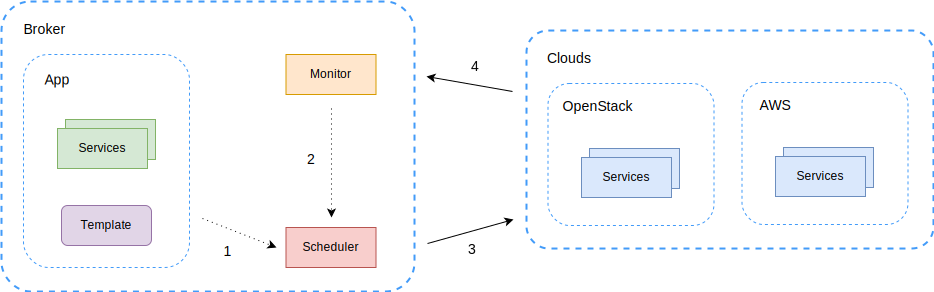
\includegraphics[width=\linewidth]{images/broker-cycle}
	\caption{Arbeitsweise des Multi-Cloud-Brokers als Zyklus: (1) Sammeln der Meta-Informationen alle Cloud-Provider, (2) Sammeln der Laufzeitinformationen der Anwendungen, (3) Sammeln der SLAs, (4) Nutzeränderungen: Neue Anwendungen oder Anpassung von SLAs, (5) Optimierungsplanung, (6) Planausführung auf den Cloud-Infrastrukturen}
	\label{fig:cycle}
\end{figure}

%Zyklus\autoref{fig:cycle}:

%\begin{description}
%	\item[Nummerierte Aufzählung]~\par
\begin{enumerate}
	
	\item Sammeln der Meta-Informationen alle Cloud-Provider
	\begin{enumerate}
		\item Kapazität (CPU, RAM, HDD, Network)
		\item Features (Verschlüsselung, CUDA, …)
		\item Geo-Lokation 
		\item Preis
	\end{enumerate}
	
	\item Sammeln der Laufzeitinformationen der PaaS/Anwendungen
	\begin{enumerate}
		\item Auslastung
		\item Fehler
		\item Ausfälle
	\end{enumerate}
	
	\item Sammeln der SLAs
	\begin{enumerate}
		\item Policy-Definitionen
		\item Policy-Konfiguration
		\item Placement-Algorithmen
	\end{enumerate}
	
	\item Neue Anwendung/Änderung eines SLA
	
	\item Optimierung
	\begin{enumerate}
		\item Feste Vorgaben (Geo, Backup)
		\item Weiche (Preis, Latenz, Verfügbarkeit)
	\end{enumerate}
	
	
	\item Ausführung
	\begin{enumerate}
		\item Netzwerkkonfiguration
		\item Allokation/De-Allokation von Ressourcen
		\item Deployment
		\item Migration
		\item Logging/Benachrichtigung
		\item Backup
	\end{enumerate}
	
\end{enumerate}

\section{Brokering}


%https://de.wikipedia.org/wiki/Constraintprogrammierung
%https://de.wikipedia.org/wiki/Scheduling

%entailing multiple constraint satisfaction (MCS)
%
%\todo{Schaubild, was wird wann gematcht}
%% Pseudocode des Algorithmus, wie in Meryn
%
%Kostenoptimierung
%
%Preisentwicklung? 
%
%Migration je nach Tageszeit? 
%
%Kosten der Datentransfers 
%
%Subscription On-Demand/Monthly/Yearly 
%
%Kompliziert durch undurchsichtige Staffelpreise
% https://www.rightscale.com/blog/cloud-cost-analysis/aws-vs-azure-vs-google-cloud-pricing-compute-instances

%https://www.rightscale.com/blog/cloud-cost-analysis/comparing-cloud-instance-pricing-aws-vs-azure-vs-google-vs-ibm

%
%Cost Calculators 
%
%http://go.appscale.com/cloud-cost-calculator-help 
%
%https://github.com/ifosch/accloudtant 
%
%https://awstcocalculator.com/# 
%

\section{Testumgebung: OpenStack \& Hyrise-R}

Hyrise\footnote{\url{https://hpi.de/plattner/projects/hyrise.html}} ist eine In-Memory-Forschungsdatenbank der Fachgruppe \emph{Enterprise Platform and Integration Concepts (EPIC)} am Hasso-Plattner-Institut \cite{grund:2010:hyrise}. Die Datenbank teilt sich einige Eigenschaften mit \emph{SAP HANA}\footnote{\url{https://www.sap.com/products/hana.html}}: Ein \emph{Delta Store}, spaltenorientierte Speicherung, Wörterbuchkodierung und weitere Komprimierungstechniken sowie den \emph{Insert-Only}-Ansatz und Partitionierung. Herausragend ist die OLAP-Performance, enthalten sind aber auch Optimierungen für OLTP-Aufgaben.

Hyrise-R ist eine Erweiterung des Basisprojektes um Replikation \cite{schwalb:2015:hyrise-r}. Es folgt dabei dem \emph{Scale-Out}-Ansatz: Alle schreibenden Operationen werden auf einem einzigen \emph{Master-Node} durchgeführt. Dessen Datensatz wird in weniger als einer Sekunde (\emph{lazy}) mit beliebig vielen \emph{Replica-Nodes} abgeglichen. Diese Spiegelungen bearbeiten alle reinen Leseanfragen und machen den Verbund so skalierbar, siehe \autoref{fig:hyrise-r}. Nach dem \emph{CAP-Theorem} sind Verfügbarkeit und Partitionstoleranz hier also wichtiger als Konsistenz. 

	\begin{figure}[ht]
	\centering
	\def\svgwidth{0.95\textwidth}
	\includesvg{images/hyrise-r}
	\caption{Verteilte \emph{Hyrise-R}-Architektur mit getrennter Verarbeitung von Lese- und Schreibanfragen. Der Master-Knoten dient als \emph{Single Source of Truth}. Zur Leistungssteigerung übernehmen Spiegelserver die Beantwortung der meisten Leseanfragen. Kleinere Inkonsistenzen werden dabei in Kauf genommen. Aus \cite{ssiclops:d42:experiments-measurements}.}	
	\label{fig:hyrise-r}
\end{figure}

Durch die verteilte Architektur ist Hyrise-R ein potenzieller Kandidat als Testanwendung innerhalb der Multi-Cloud-Umgebung. Einige \emph{SSICLOPS}-Teilprojekte untersuchten bereits Zuverlässigkeit, Performance, Datensicherheit und Vertraulichkeit in einer privaten OpenStack-Föderation \cite{ssiclops:d23:security-extensions, ssiclops:d42:experiments-measurements, bastian:2017:openstack-policies}. \todo{Diagramm:Hyrise-R on SSICLOPS}

Im Rahmen dieser Arbeiten sind einige Infrastrukturteile als Code veröffentlicht: So existiert zum Beispiel eine Docker-Teststellung mit grafischem Cluster-Manager, um die Performance bei verschiedenen Replikationsstufen zu prüfen. Diese Infrastruktur wurde in mehreren Studienarbeiten weiter angepasst, um Hyrise-R-KVM-Images in OpenStack bereitzustellen \cite{eschrig:2016:ssiclops-masterproject, maschler:2017:ssiclops-masterproject}. Möglicherweise können Teile dieser Arbeiten weiterentwickelt werden.


\input{content/4-4_openstack-testbed.tex}

\input{content/4-5_devstack-docker.tex}

\input{content/4-6_multi-cloud-bibliotheken.tex}


\section{Entwicklungsumgebung}

% Hyrise-R-OpenStack- und Docker-Images, wie ersxtellt?

%Bestehende verteilte Anwendungen für den EInsatz in der CLoud vorbereiten, STichwort CLoud Native.
%Ausgangslage? Git-Repository mit teilautmatisierten Shell-Skripten und Makefiles. Automatisierung der Build, Test und Produktions-Infrastruktur, Ubuntu 16.04 auf Bare-Metal, VM und (Docker)Container.
%Integrieren der bestehenden Tests in diese Umgebungen.
%Packen des Geamtpakets aus Ausführungsumgebung, Programm und (Test-)Daten. auch automatisiert. Die Konfiguration ist variabel. SIe wird schematisch in der App-Konfiguration vorgegeben und dann von der CMP während der initialen Bereitstellung oder späteren Re-Deployments angepasst und ausgeführt.

% Tatsächliche Broker Architektur
% Code-Eigenheiten
% Tests/KPIs/Validierung der Hypothese

\section{Softwarearchitektur}

%as in Grozev 42: Federated CLoud Management: There is a central repository of images. this is replicated to the specific iaas/caas providers on demand.
%
%Alle weiteren Managementprozesse sind für Clients transparent.


\section{Multi-Provider-Service-Schema}

% D2.1: Übersicht Policy-Sprachen: Performance und Speichergröße. Entgegengesetzte Interessen. Lesbarkeit über zweiteiliung: Einmal für Menschen, einmal auf Bit-ebene für Maschinen. SLA über Proxy

%D2.2: Policys auf allen Schichten

%Matthias Bastian: Policy in OpenStack.

...und SLAs.

Ziel: Portabilität.

Mensch-und maschinenlesbar

YAML als aktuellen Standard

%TOSCA komplex, aber vielversprechend. Hierauf aufbauen (eigenen YAML-Entwurf erwähnen) und Brokering hinzufügen. Hier muss festgelegt erden, welcher Service-Teil auf welchem Provider mit welchem Instanz-Typen bereitgestellt werden soll. Dies soll automatisiert anhand von SLA/Policy und Preis entschieden werden. Unterstützt TOSCA deklarative Service-Definitionen?
%
%
%TOSCA hat folgendes nur optional
%- YAML (als SimpleVersion)
%- Multi-Provider als Plugin (nicht gewartet)
%- 
\begin{listing}[ht]	
	\inputminted[]{yaml}{./src/provider.sample.yaml}
	\caption{Provider-Definition und Zugangsdaten. Der Broker liest alle eingetragenen Accounts automatisch ein und berücksichtigt sie bei der initialen Service-Bereitstellung sowie in Optimierungsläufen. Public-Clouds benötigen nur Zugangsdaten wie Benutzername und Passwort -- alle weiteren Informationen erfragt der Broker dynamisch zur Laufzeit vom Provider. In Private-Cloud-Umgebungen ist dies nicht immer möglich: Details zur Verfügbarkeit, geografische Lage und Kosten müssen manuell eingepflegt oder vom Monitoring festgestellt werden.}
	\label{listing:provider}
\end{listing}



Platzhalter werden mit Jinja während des Deployments gefüllt.

Ablage der Pläne als Dokumentation.

Broker durch Metainformationen (und Labels) der Instanzen theoretisch zustandslos -> Broker selbst ist nicht ausfallgefährdet.

Erklärung der Metainformationen (versionierbar), verschiedenen Parameter und Rollenbeschreibung.

Je Provider Angaben zu Image und Startkommando. Dies wird hier eingetragen, um vom Broker dynamisch mit aktuellen Variablen angepasst zu werden: IP, Port...

Abhängig vom Service Level: IaaS/CaaS. Auch PaaS ist so denkbar. (Angabe als Image, Interpretation durch den Broker)

Beispiel verlinken.
Kapitel: Legacy Services Hyrise

Image-Erstellung und Repository.

Eigene Befehle
- Cloud-Init (Standard)
- shell/bash (Docker)

Vordefinierte Policys z.B. zum Verhalten im Fehlerfall. Aber auch Zusatzinformationen: Wie ist die Zustandsprüfung auf Service-Ebene auszuführen. Wichtig für Monitoring der Verfügbarkeit (SLA).

Abhängigkeiten von Services und wie oft global vorhanden? Hier: global ein master, abhängig vom Dispatcher.

\begin{listing}[ht]	
	\inputminted[firstline=15]{yaml}{./src/hyrise-r.sample.yaml}
	\caption{Providerübergreifende Servicevorlage. Der Ausschnitt zeigt die Definition des zentralen \emph{Hyrise-R-Dispatcher}-Dienstes. Nicht zu sehen sind Metadaten und die übrigen Anwendungsbestandteile. Parameter werden zur Laufzeit vom Broker eingesetzt.}
	\label{listing:hyrise-r}
\end{listing}

Könnte auch zu einem konkreten CAMP-Plan umgewandelt werden. So wie TOSCAMP. Stattdessen nur ein Template Schema und Graph zur Laufzeit.
%https://brooklyn.apache.org/v/latest/blueprints/setting-locations.html


\section{Tests und Diskussion}

%Kosten: Rechenzeit und Bandbreite (außerhalb einer Cloud) also gegenläufiges Ziel zu Portabilität und Ausfallsicherheit, denn die geringsten Kosten fallen bei dem Betrieb in einer einzelnen Cloud eines Providers an.
%i) providers’ pricing models, (ii) application’s communication patterns and (iii) distribution of nodes over providers.
%https://www.google.de/url?sa=t&rct=j&q=&esrc=s&source=web&cd=1&ved=0ahUKEwju27vHs6DZAhUCWRQKHRv7BEcQFggrMAA&url=http%3A%2F%2Fwww.mikesmit.com%2Fwp-content%2Fpapercite-data%2Fpdf%2Fcloud2012.pdf&usg=AOvVaw3e6yhHYmhWBbIxtr7MqkuX

%verschiedene OpenStack-Versionen haben unterschiedliche Schnittstellen. Auch dies kann über die Middleware abgefangen werden. RefStack testet API, Rally testet performance und führt tempest-Tests aus.


Aufwand einer Multi-Cloud-Strategie

Umsetzung der Policys

Potential

Vorteile durch Multi-Cloud-Bibliotheken

Aufwand für ein Multi-Cloud-Testbed
	%In der Schlussbetrachtung gibt es einen Rückblick, in dem Motivation und Thesen aus der Einleitung wieder aufgegriffen und abgerundet werden. Antworten auf in der Problemstellung aufgeworfene Fragen werden kurz und prägnant zusammengefasst. Ebenso sollte ein Ausblick auf offen gebliebene Fragen sowie auf interessante Fragestellungen, die sich aus der Arbeit ergeben, gegeben werden. Ein persönlich begründetes Fazit aus eigener Perspektive ist an dieser Stelle ebenfalls sinnvoll.
%

\chapter{Zusammenfassung und Ausblick}

\begin{description}
	
	\item[Notfallplan] Bei Ausfall der gesamten Ausführungsplattform kann eine Migration zu einem anderen Anbieter erfolgen.
	
	\item[Abfangen von Lastspitzen] Zusätzliche Service-Instanzen auf externen Ressourcen bearbeiten bei Bedarf weitere Anfragen.
	
	\item[Lebenszyklus-Verwaltung] Typischerweise durchläuft eine neue Service-Version die Phasen Entwicklung, Test, Qualitätssicherung und Produktion. Hierfür existieren oft unterschiedliche Ausführungsumgebungen.
	
\end{description}

%Rightscale Video: https://www.rightscale.com/solutions/problems-we-solve/self-service-it

Einheitliche Standards zu Services, SLAs und Kommunikation.

Policys innerhalb von Instanzen 
%(allow SSH, check for security vulnerabilities)

Policys auf Datenebene

Ausbau zu einer produktiven CMP
Identity
Discovery
Monitoring
Dashboard
CAMP-Pläne zum Austausch mit weiteren Cloud-Management-Plattformen.

Trend: Serverless

Migrationshürden von Apps auf die CMP: OS Version, SSL-Zertifikate, statische und virtuelle IPs, Lizenzen, Load Balancing, Clustering, Bandbreite, Mandantenfähigkeit.

Failover-Handling nicht definiert. Im Moment: Bereitstellung eines Services mit der gleichen Adresse bei Ausfall. Weitere Arbeit auf Anwendungsebene (Hyrise-R) nötig. Oder Ausgliederung der Service-Discovery an ein externes Tool.

Überwachung der SLAs und Durchsetzen von Schadensersatz.
	
	% Bibliographie
	\ifisbook\cleardoubleemptypage\fi
	\phantomsection\addcontentsline{toc}{chapter}{\refname}
	\printbibliography[category=cited]

	% Eigenständigkeitserklärung
	\ifisbook\pagestyle{plain}\cleardoubleemptypage\include{content/disclaimer}\fi

\end{document}